\documentclass[english]{beamer}
\mode<presentation>

%\usepackage[slovak]{babel}
\usepackage[utf8]{inputenc}
\usepackage{physics}
\usepackage{tikz, pgfplots}
%\DeclareMathSizes{12pt}{10pt}{10pt}{10pt}

\usepackage{multimedia}
\RequirePackage{environ}

\usepackage{changepage}
\makeatletter
\newenvironment{forcecenter}%
    {\@parboxrestore%
     \begin{adjustwidth}{}{\leftmargin}%
    }{\end{adjustwidth}
     }
\makeatother

%\graphicspath{images}

%Use Okular!

\newcommand\Wider[2][3em]{
\makebox{\linewidth][c]{
	\begin{minipage}{\dimexpr\textwidth+#1\relax}
	\raggedright#2
	\end{minipage}	
	}
}
}

\NewEnviron{sea}{
	\fontsize{9}{12}
    \begin{eqnarray*}
   % \fontsize{12pt}{10pt}\selectfont
    \BODY
    \end{eqnarray*}
    \normalsize
}

\begin{document}

  \title{Explaining symmetry elevation in InGaAs quantum dots through bulk symmetry-structure symmetry interaction}
  \author[Michal Horanský]{Michal Horanský\\\hfill\\Imperial College London}
  %\date{14. apríl 2019}
  %\maketitle
  \date{January 10, 2024}
  \begin{frame}
    \titlepage
  \end{frame}
    %\begin{center}
    %\includegraphics<1->[scale=0.5]{images/multipendulum_scheme.png}
    %\end{center}
  
  
  \begin{frame}
  	\frametitle{Introduction}
  	\framesubtitle{An outline of the problem}
  	\begin{itemize}
  		\item Master's project (MSci) under Professor Dimitri Vvedensky at Imperial College London
  		\item Collaboration with Professor Stefan Schulz and Professor Emanuele Pelucchi
  		\item Problem specifics:
  		\begin{itemize}
  		\item Quantum dots with high spatial symmetry: photoluminiscence
  		\item Fine-structure splitting of excitonic energy levels
  		\item Resolvable peaks within major features of the photoluminiscence spectrum
  		\item Symmetry elevation
  		\end{itemize}
  		\item Motivation:
  		\begin{itemize}
  		\item Artificial atoms
  		\item Programmable structural and spectral properties
  		\item Usage in quantum computing, medical imagining, lasing, photovoltaic engineering, and other areas.
  		\end{itemize}
  	\end{itemize}
  \end{frame}
  
  \begin{frame}
  	\frametitle{Introduction}
  	\framesubtitle{The quantum dot in question}
  	
  	\begin{figure}
	\centering
    		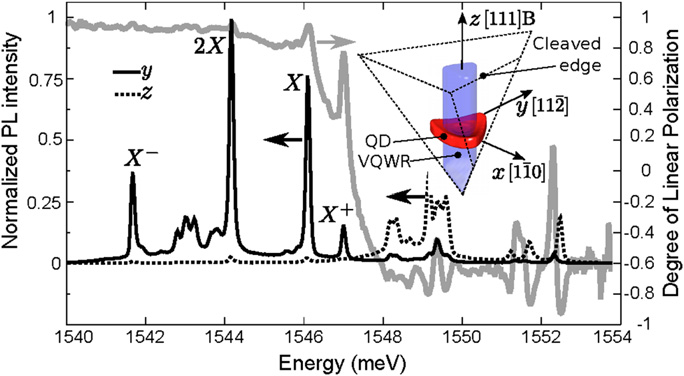
\includegraphics[width=0.9\textwidth]{images/QD_schematic}
    		\caption{Gross spectrum of a $C_{3v}$ InGaAs QD. Image credit: Karlsson, K. F. et al (2015), Spectral signatures of high-symmetry quantum dots and effects of symmetry breaking. New Journal of Physics, 17 103017}
    		\label{fig:qd}
	\end{figure}
\end{frame}

	\begin{frame}
		\frametitle{Introduction}
		\framesubtitle{Exciton energy levels and transitions}
		\begin{figure}
	\centering
    		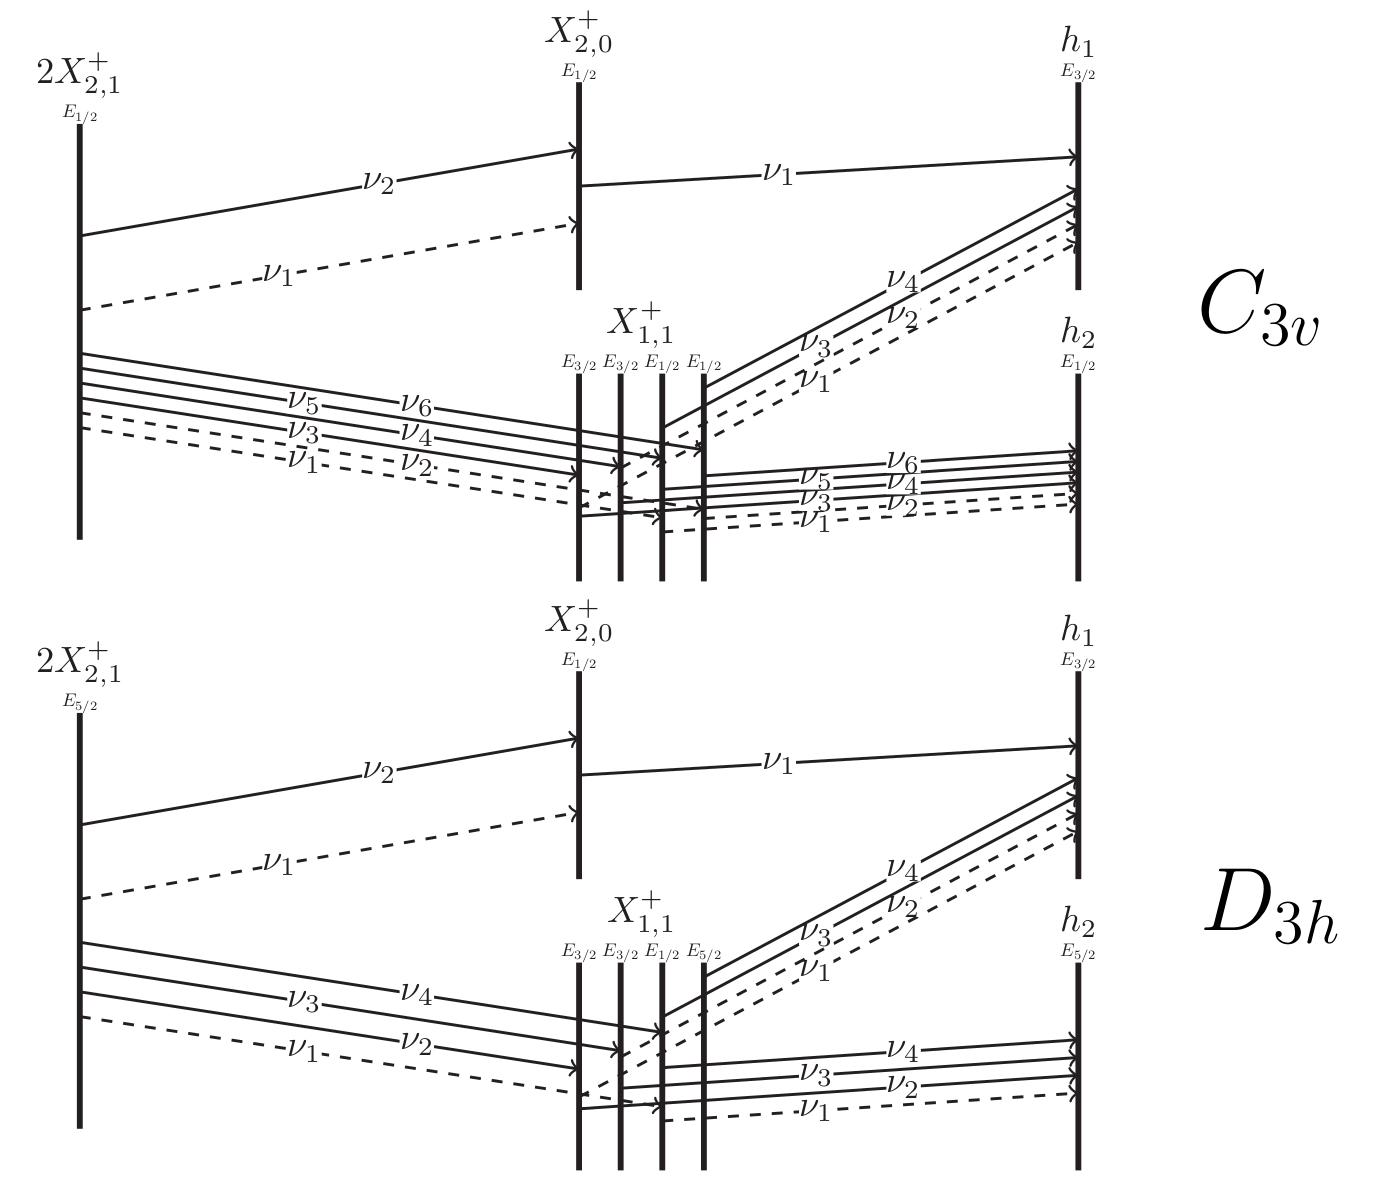
\includegraphics[width=0.85\textwidth]{images/2X21_scheme}
    		\label{fig:qd}
	\end{figure}
		
	
	
	\end{frame}
  
  \begin{frame}
  	\frametitle{Results}
  	\framesubtitle{Framework for automatic energy level splitting and selection rules calculation}
  	\begin{itemize}
  		\item Structure point group is a subgroup of $SU(2)\otimes C_i$
  		\item Single fermions are $j$-eigenstates, hence we can use subduction
  		\item Multiplication tables of double groups can be constructed from the double covering of $O(3)$ by $SU(2)\otimes C_i$ (quaternion approach)
  		\item The faithful irrep of $SO(3)$ is the Cartesian rep, which, subdued into the double group, identifies the Cartesian basis vector transformation laws.
  		\item By considering subtraces of Wigner D-matrices, we can identify the irreps and basis partners of any $j$-state $\ket{j,m}$.
  		\item A careful treatment of parity under $l$- and $j$-coupling is introduced.
  		\item The entire group-theoretical analysis as performed by Karlsson et al. is automated in our Python package AReTDoG (Algorithms for Representation Theory of Double Groups).
  	\end{itemize}
  \end{frame}
  
  \begin{frame}
  	\frametitle{Results}
  	\framesubtitle{Symmetry suppression theory}
  	\begin{itemize}
  		\item Symmetry elevation can be understood as partial symmetry breaking from a higher-symmetry Hamiltonian $\hat{H}_+$ which approximates the true Hamiltonian $\hat{H}$.
  		\item Every eigenstate of $\hat{H}$ decomposable into an eigenstate of $\hat{H}_+$ and a residual component.
  		\item Surjection of basis vectors $\rightarrow$ transformation properties of the elevated symmetry component
  		\item Selection rules can allow a transition from the lower symmetry eigenstate but forbid it from the elevated symmetry component, suppressing the rate.
  	\end{itemize}
  \end{frame}
  
  \begin{frame}
  	\frametitle{Results}
  	\framesubtitle{Evidence for symmetry suppression in InGaAs QDs grown in inverted tetrahedrons}
  	\begin{itemize}
  		\item Symmetry elevation matches the bulk symmetry ($C_{6v}$) on a sample dataset.
  		\item Differently-sized quantum wires in the growth mode result in a hexagonal structure.
  		\item By considering only the envelope functions, we model exciton complexes as a many-body particle system in a box with $j$-coupling and Coulomb interactions.
  		\item Wavefunction localisation around the centre--approximate elevation from structure symmetry to bulk symmetry.
  		\item Due to breakage of exchange symmetry, mixed-hole excitons are predicted to probe for structure symmetry.
  		\item Pure light-hole excitons empirically probe for structure symmetry, presumably due to weak localisation in the centre.
  	\end{itemize}
  \end{frame}
  
  \begin{frame}
		\frametitle{Results}
		\framesubtitle{Evidence for symmetry suppression in InGaAs QDs grown in inverted tetrahedrons}
		\begin{figure}
	\centering
    		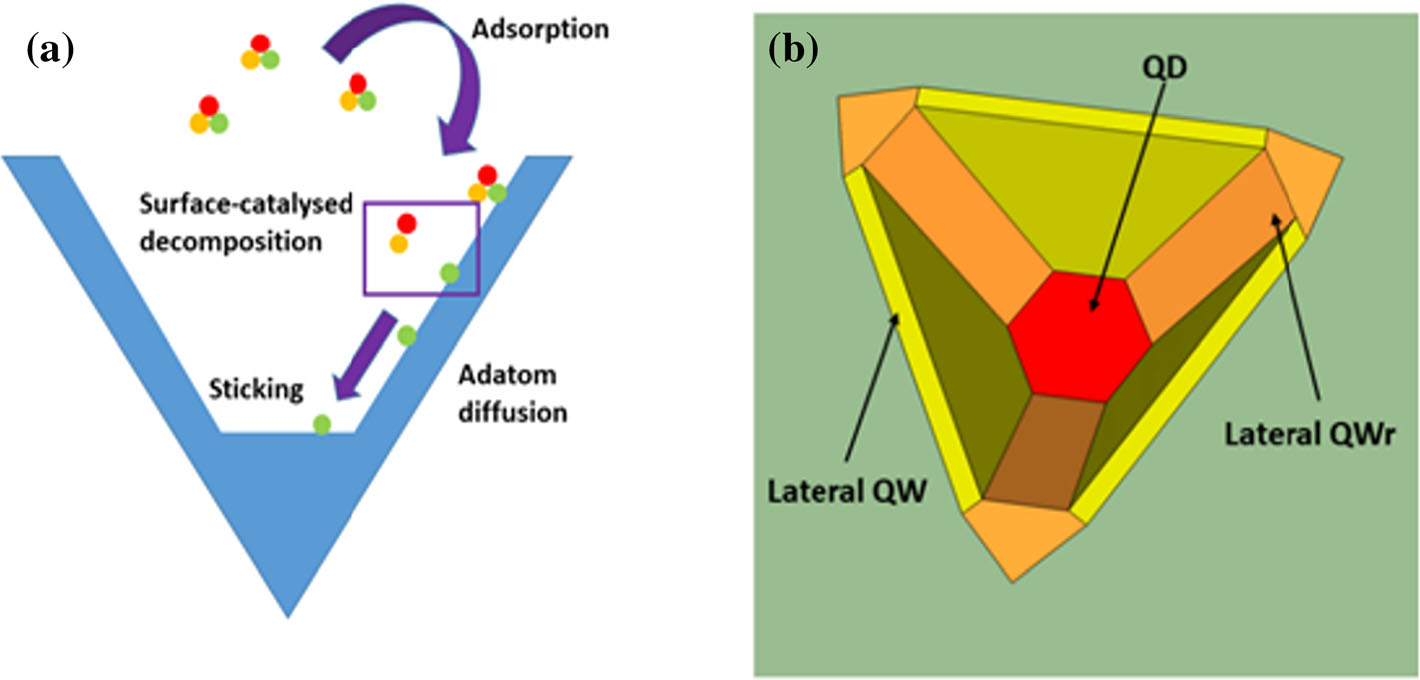
\includegraphics[width=0.85\textwidth]{images/MOVPE_process}
    		\label{fig:growth}
    		\caption{The epitaxy growth process and the sketch of a QD with large-scale QWs. Smaller QWs may result in an irregular hexagon with 3+3 structure. Image credit: Holsgrove, K. M. et al (2022), Towards 3D characterisation of site-controlled InGaAs pyramidal QDs at the nanoscale. J Mater Sci., 57:16383--16396}
	\end{figure}
  \end{frame}
  
  \begin{frame}
  	\frametitle{Predictions and outlook}
  	%\framesubtitle{MSci third-year group project at ICL}
  	\begin{itemize}
  		\item We predict only pure heavy-hole excitons to undergo symmetry elevation to bulk symmetry (weakly supported by Karlsson data)
  		\item An error in Karlsson analysis of $C_{6v}$ selection rules--$C_{6v}$ and $D_{3h}$ do give different predictions regarding the $z$-polarised spectra.
  		\item We predict one weak $z$-polarised emission line for every pure heavy-hole exciton complex (challege in identification).
  		\item We also predict pure light-hole excitons to be delocalised in the QD.
  		\item These predictions will be compared to experimental data (Pelucchi) as well as simulation (Schulz).
  	\end{itemize}
  \end{frame}
  
  \begin{frame}
  	\frametitle{References}
  	\begin{itemize}
  		\item García de Arquer, F. P. \textit{et al} (2021), Semiconductor quantum dots: Technological progress
and future challenges. \textit{Science}, \textbf{373}, 640
		\item Karlsson, K. F. \textit{et al} (2015), Spectral signatures of high-symmetry quantum dots and effects of symmetry breaking. \textit{New Journal of Physics}, \textbf{17} 103017
		\item Holsgrove, K. M. \textit{et al} (2022), Towards 3D characterisation of site-controlled InGaAs pyramidal QDs at the nanoscale. \textit{Journal of Materials Science}, \textbf{57} 16383--16396
		\item Dresselhaus, M. S. (2002), \textit{Applications of Group Theory to the Physics of Solids.} Massachusetts Institute of Technology
		\item Burt, M. G. (1999), Fundamentals of envelope function theory for electronic states and photonic modes in nanostructures. \textit{Journal of Physics: Condensed Matter}, \textbf{11} 53
  	\end{itemize}
  
  \end{frame}
  

\end{document}